\chapter{Basic concepts in complexity theory}

The fundamental question driving the study of computational complexity theory
is, ``how difficult are certain problems for computers to solve?''  In order to
answer this question precisely, we must start by figuring out what exactly it
asks.  That is, formally, what do we mean by \emph{difficulty}?  For that
matter, what constitutes a \emph{problem}?  What counts as a \emph{computer}?

Conventionally, \emph{computers} are formalized as Turing machines, with
\emph{difficulty} being measured by the number of Turing machine execution
steps.  For the purposes of this thesis, we avoid delving into the formalism of
Turing machines.  Instead, we assume an informal notion of computers given by
any algorithm or procedure straightforwardly implementable in modern,
high-level programming languages such as C/C++, Python, Java, etc.  Detailed
treatment of the relevant formalisms may be found in \textcite[Chapter
2]{papadimitriou.cc}.  In particular, there are theorems \parencite[Theorem
2.5]{papadimitriou.cc} showing that modern CPU/RAM-based computer architectures
are, for our purposes, equivalent to Turing machines, thereby justifying the
informal approach we take here.

In the following sections, we discuss what exactly constitutes a
\emph{problem}, how we describe the complexity (i.e., difficulty) of problems,
and how we categorize problems by difficulty into \emph{complexity classes}.

%emphasize intuitive descriptions of
%algorithms in terms of modern, ``high-level'' programming concepts exhibited by
%programming languages such as Python.

%An
%alternative treatment uses ``random access machines'', which mimic modern
%CPU/RAM-based computer architectures.  In this thesis, we avoid delving into
%these formal details.

%in terms of modern, high-level programming concepts

%In the conventional formalism, computers are modeled as Turing machines.
%Difficulty, then, refers to the number of execution steps required by a Turing
%Machine to solve a problem.  Alternatively, computers could be modeled as
%``random access machines'' \parencite[Section 2.6]{papadimitriou.cc}, which
%mimic modern CPU/RAM-based computer architectures.  For our purposes, the two
%models of computation are equivalent \parencite[Theorem 2.5]{papadimitriou.cc}.

%Formal treatments of these
%definitions are found in \textcite[Chapter 2]{papadimitriou.cc}

%Of particular
%note, \textcite[Theorem 2.5]{papadimitriou.cc} shows that these two models of
%computation are, for our purposes, equivalent.  Therefore, for our purposes, we will
%assume the latter model, allowing us to think in terms of modern programming
%patterns and give

%By \emph{hardness}, what we really mean is: given a problem input
%encoded in \(n\) bits, how much computational time, asymptotically with respect
%to \(n\), is required to solve that problem?  In order to discuss this question
%precisely, we have to clearly define what we mean by ``computational time'',
%and, for that matter, what we mean by ``computer''.  A traditional approach
%takes ``computer'' to mean Turing Machines and ``time'' to be Turing Machine
%execution steps; another approach defines ``computer'' via modern-day,
%CPU/RAM-based architectures, with ``time'' given by CPU instruction cycles.

%relatively \emph{informal} descriptions of algorithms.

\section{Decision problems}

The simplest flavor of computational problem is a \emph{decision problem}, or a
yes/no question: given an input \(X\), does \(X\) satisfy certain conditions?
Here are some examples of decision problems:
\begin{itemize}[nosep]
  \item Given an integer \(K\), is \(K\) even?
  \item Given a string of letters \(S\), is \(S\) a palindrome?
  \item A silly decision problem, but nevertheless a valid one: given any input
    \(X\), always return ``yes''.
\end{itemize}

In order for a yes/no question to qualify as a decision problem, it must be
stated in terms of an arbitrary input.  For instance, consider the following
question:
\begin{itemize}[nosep]
  \item Is \(314159\) a prime number?
\end{itemize}
This is a yes/no question, but it takes no inputs (the value \(314159\) is not
an input; it is merely part of the question statement).  In this sense, it is
computationally uninteresting: in order to solve this question, an algorithm
only needs to return the fixed answer ``yes''.  In contrast, what we're really
interested in is the general problem of primality testing:
\begin{itemize}[nosep]
  \item Given an arbitrary positive integer \(K\), is \(K\) prime?
\end{itemize}

We formalize the definition of decision problems below.

\begin{definition}{(decision) problem}{}

  A \Term{decision problem} is a function
  \(Π\colon\Set{0,1}^*→\Set{\text{yes},\text{no}}\).  Equivalently, a
  \Term{decision problem} is the set \(Π⊆\Set{0,1}^*\) comprising exactly the
  inputs, a.k.a. \Term{instances}, that result in ``yes'' answers.

  That is, for any input \(X∈\Set{0,1}^*\), we say \(X∈Π\) (in the \emph{set}
  sense) if \(Π(X)=\text{yes}\) (in the \emph{function} sense), and \(X∉Π\) to
  mean \(Π(X)=\text{no}\).  The two formalisms are equivalent.

  \begin{aside}
    Formally, inputs to decision problems are always encoded as binary strings.
    Essentially, this requirement follows from the fact that all modern
    computers encode data in binary anyway.  Furthermore, it allows us to
    rigorously discuss notions such as \emph{input size}.  This is an important
    formal detail, but for the most part, we avoid dealing with any binary
    encoding/decoding technicalities.  We mention this detail here only to
    clarify the role of \(\Set{0,1}^*\) in the definition above.
  \end{aside}

\end{definition}

A more general notion of \emph{problems} considers arbitrary (binary-encoded)
functions \(\Set{0,1}^*→\Set{0,1}^*\); such a problem is termed a \Term{function
problem}.  However, we will focus mainly on decision problems for two reasons.
First, decision problems are easier to work with than function problems. Second,
function problems can be encoded in terms of decision problems (e.g., mapping
each output bit to its own decision problem).  Essentially, the \emph{decision
problem} formalism is conceptually simpler but remains versatile enough to
capture the important core ideas of complexity theory. As such, the vast
majority of the problems examined in this thesis are decision problems. For
convenience we will simply say ``problems'' to mean decision problems, unless
otherwise specified.

\section{Complexities and classes}

When we ask how difficult a problem is, we are essentially asking, how much
time (or other resources, such as memory) does a computer need to solve that
problem?  Of course, the answer depends on the input: some inputs are easy to
solve, and others are harder.  Certainly, we expect the difficulty to scale
with input size: the larger the input, the more work it generally takes an
algorithm to process it.  Thus, the complexity of a problem is given as a
function of the input size.  Specifically, we ask, if an algorithm is given an
input string (recall, encoded in binary) of length \(n\), how much time in the
worst case is required, as a function of \(n\)?

However, exact function bounds are unnecessarily sensitive to pedantic
technicalities, e.g., slight variations in implementations of the same
algorithm, or specific details in the formal models of ``computer''. Instead,
loosely speaking, we are mostly interested in how these costs asymptotically
\emph{scale} as the input size gets large.  Thus, we categorize problems with
``similar'' complexities into \emph{complexity classes}.

So then, what counts as \emph{similar}?  As a starting approximation, we assert
that \emph{polynomials are small}: any algorithm whose running time is bounded
by some polynomial function is considered relatively ``fast''; problems with
polynomial-time solutions are considered relatively ``easy''.  We formalize
this idea in the definition of the complexity class \P{} below.

\begin{definition}{Polynomial-time problems, \P}{}

  Let \(A\) be an algorithm computing some (decision) problem (i.e., it takes a
  binary string as input and returns ``yes'' or ``no'').  We say \(A\) runs in
  \Term{polynomial time} if there exists some polynomial \(p\) such that, on
  any input \(X∈\Set{0,1}^*\), the algorithm \(A\) \emph{always} terminates in
  \(≤p(\Abs X)\) steps.

  The complexity class \P{} is the set of (decision) problems correctly
  solvable in polynomial time.

  \begin{aside}
    For contrast, we say an algorithm is \Term{super-polynomial} if its running
    time cannot be bounded by some polynomial.  Examples of super-polynomial
    functions include \(n^{\log n}\), \(2ⁿ\), etc.
  \end{aside}

\end{definition}

To be clear, taking polynomials to mean ``easy'' is a very crude rule-of-thumb:
there are important practical subdivisions \emph{within} \P{} that this
categorization plainly ignores (e.g., linear-time vs quadratic-time); there are
also a few notable examples of super-polynomial-time algorithms that are, by
this rule, slow, but quite efficient \emph{in practice} (e.g., the simplex
algorithm for linear programming).  Nevertheless, this delineation remains an
extremely useful (and arguably elegant) starting point for the classification
of problems.

\subsection{How to tell when an algorithm is polynomial-time}

TODO: examples of \P{} problems, some basic facts and intuition about closure
of polynomials under multiplication, composition, etc.

ALSO TODO for earlier: may need to briefly remark on what's allowed as
algorithm, i.e. determinism, no randomness, etc.

% TODO examples of 𝐏 problems, and perhaps discuss papadimitriou theorem 2.5
% again with more precision?

\section{Hard problems and reductions}

Above, we establish that a problem is considered \emph{easy} if it has a
polynomial-time solution.  Hard problems, then, are those without
polynomial-time solutions… right?  Sure.  But how do we go about showing that a
problem is actually hard?  And how hard, exactly?

For an easy problem, proving \emph{existence} of a polynomial-time algorithm is
straightforward---simply construct one.  On the other hand, for a problem that
appears to be hard, we would have to prove \emph{non-existence} of a
polynomial-time algorithm---that it is \emph{impossible} to find a
polynomial-time algorithm. In general, this is incredibly difficult to show;
this difficulty is largely why the infamous \P-vs-\NP{} question remains
unsolved.

Instead, we take a different approach to understanding hard problems: comparing
them to each other.  To illustrate, consider the following two problems:

\begin{description}

\item[\Problem{Latin Square}] Given a square grid of dimensions \(n×n\) (for
  some \(n\)), with some of its cells filled in with a number in
  \(\Set{1,\dotsc,n}\), is it possible to complete the remaining cells so that
  each row and each column contains each number exactly once?

  \begin{figure}[H]
    \begin{center}
      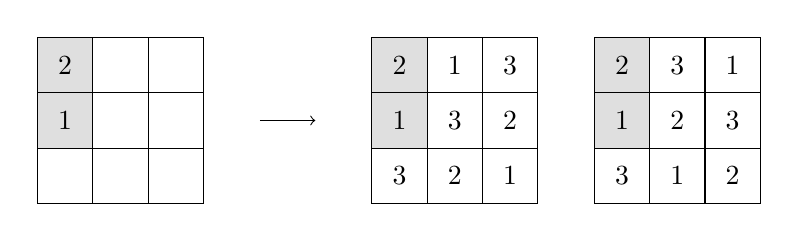
\begin{tikzpicture}[x=2em, y=2em]

        \tikzset{
          ls/.pic={
            \draw
            (0,0) rectangle (3,3)
            foreach \i in {1,2} { (0,\i) -- +(3,0) (\i,0) -- +(0,3) };

            \foreach \i/\j/\n in {0/2/2,0/1/1} {
              \fill[opacity=1/8] (\i,\j) rectangle +(1,1);
              \node at (\i+1/2,\j+1/2) {\(\n\)};
            };
          },
          lss/.pic={
            \pic{ls};
            \node at (1/2,1/2) {\(3\)};
            \foreach \i in {0,1,2} {
              \pgfmathtruncatemacro\m{Mod(\i+#1-1,3)+1}
              \pgfmathtruncatemacro\n{Mod(\i-#1-1,3)+1}
              \node at (1+1/2,\i+1/2) {\(\m\)};
              \node at (2+1/2,\i+1/2) {\(\n\)};
            }
          },
        }

        \matrix[column sep=2em] {
          \pic{ls}; & \draw[->] (0,3/2) -- +(1,0); &
          \pic{lss=-1}; & \pic{lss=1}; \\
        };

      \end{tikzpicture}

      \caption{A \(3×3\) Latin Square instance and its two possible
      completions.}

      \label{fig:background.latin-square-example}

    \end{center}
  \end{figure}

\item[\Problem{Graph Coloring}] Given a positive integer \(k\), and a graph
  with \(n>k\) vertices, some of which are assigned a number (a.k.a. ``color'')
  in \(\Set{1,\dotsc,k}\), is it possible to assign numbers to the remaining
  cells so that no neighboring vertices receive the same assignment?

  \begin{figure}[H]
    \begin{center}
      \begin{tikzpicture}


      \end{tikzpicture}
    \end{center}
  \end{figure}


  TODO diagram illustrations.  also i wish i could think of simpler-to-state
  examples with easy reductions, but nothing comes to mind, so this is the best
  i've got for now.

\end{description}

Is one of these problems ``easier'' than the other?  In a sense, yes: the
\Problem{Latin Square} problem is just a special case of the \Problem{Graph
Coloring} problem, where the vertices are arranged into a square grid, and all
vertices in the same row or column neighbor each other.

\begin{figure}[H]
  \begin{center}
    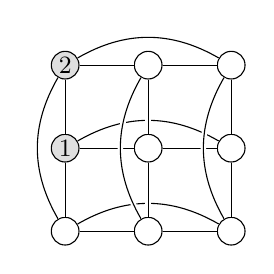
\begin{tikzpicture}[x=3em, y=3em]

      \tikzset{
        vert/.style={circle, draw, minimum size=1em, inner sep=0pt, font=\small},
        pre/.style={vert, fill, fill opacity=1/8, text opacity=1},
        edge/.style={preaction={draw=white, line width=2pt}},
      }

      \node[pre](02) at (0,2) {\(2\)};
      \node[pre](01) at (0,1) {\(1\)};
      \coordinate[vert](00) at (0,0){};

      \foreach \i in {1,2} { \foreach \j in {0,1,2} {
          \coordinate[vert](\i\j) at (\i,\j);
      } };

      \draw[edge] foreach \i in {0,1,2} { (0\i) to[bend left] (2\i) };
      \draw[edge] foreach \i in {0,1,2} { (\i0)--(\i1)--(\i2) (0\i)--(1\i)--(2\i) };
      \draw[edge] foreach \i in {0,1,2} { (\i0) to[bend left] (\i2) };

    \end{tikzpicture}

    \caption{The Latin Square from \cref{fig:background.latin-square-example},
    represented as a graph.}

  \end{center}
\end{figure}

More precisely, this argument describes a way to convert any \Problem{Latin
Square} instance (a partially-filled \(n×n\) grid) into a \Problem{Graph
Coloring} instance (a partially-colored graph with \(n²\) vertices) with the
same yes/no answer.  Formally, we call this conversion a \Term{reduction}:

\begin{definition}{reductions}{}

  Let \(Π₁\) and \(Π₂\) be decision problems.  A \Term{reduction} from \(Π₁\)
  to \(Π₂\) is an algorithm \(R\colon\Set{0,1}^*→\Set{0,1}^*\) such that, for
  each \(X∈\Set{0,1}^*\), \(X∈Π₁\) if and only if \(R(X)∈Π₂\).

  In other words, \(R\) converts problem-inputs (a.k.a. \emph{instances}) of
  \(Π₁\) to problems-inputs of \(Π₂\) such that the yes/no answers on the
  original and converted inputs exactly match.

  %\begin{aside}
  %  %This definition is sometimes called \emph{Karp reductions} or
  %  %\emph{many-one reductions}, in order to distinguish it from other notions
  %  %of reduction such as \emph{Turing/Cook reductions} and \emph{truth-table
  %  %reductions}, which are related but different.

  %  %For our purposes, Karp reductions are the simplest to describe and
  %\end{aside}

\end{definition}

Revisiting the above example, the existence of a reduction from \Problem{Latin
Square} to \Problem{Graph Coloring} captures the idea that \Problem{Latin
Square} is easier than \Problem{Graph Coloring} in the following sense.
Suppose that we already know how to solve \Problem{Graph Coloring}.  Then, we
automatically also know how to solve \Problem{Latin Square}: given an arbitrary
\Problem{Latin Square} input, apply the reduction to convert it into a
\Problem{Graph Coloring} input, feed that input into the known \Problem{Graph
Coloring} solver, then directly return its answer.

However, in order to authentically capture the idea of \emph{easiness}, we must
also account for computation time.  Namely, we stipulate that the reduction
itself must be efficient---formally, that it runs in polynomial time.

\begin{definition}{polynomial-time reducibility}{}

  Let \(Π₁\) and \(Π₂\) be decision problems.  We say \(Π₁\) is
  \Term{polynomial-time-reducible} to \(Π₂\), which we denote as
  \[
    Π₁≤Π₂,
  \]
  if there exists a reduction from \(Π₁\) to \(Π₂\) that runs in polynomial
  time.  (The \(≤\) notation evokes the intuition that \(Π₁\) is easier than,
  or \emph{at most as hard as}, \(Π₂\).)

\end{definition}

Finally, we introduce some terminology to describe how one problem compares to
a \emph{class} of problems:

\begin{definition}{hardness and completeness}{}

  Let \(Π\) be a decision problem, and let \(\C\) be a class of decision
  problems.

  We say \(Π\) is \Term{hard} for \(\C\), or \Term{\C-hard}, if every
  problem in \C{} is polynomial-time-reducible to \(Π\).

  We say \(Π\) is \Term{complete} for \C, or \Term{\C-complete}, if \(Π\) is
  \C-hard and \(Π∈\C\).

  \begin{aside}
    Following the intuition that reducibility (\(≤\)) defines a (partial)
    ordering of problems by difficulty, \C-hard problems are just those that
    are (non-strictly) harder than all problems in \C, and \C-complete problems
    are just the \emph{maximal/hardest} problems within \C.
  \end{aside}

\end{definition}

Complete problems are especially useful, first and foremost, because they are
tangible.  They have accessible, interesting, and often real-world-applicable
examples that help us understand complexity classes in concrete, intuitive
terms, rather than pure abstractions.  At the same time, complete problems are
also very general.  As \emph{tight} difficulty upper bounds of a complexity
class, they are perfect characterizations of these classes; determining the
exact difficulty of a complete problem automatically essentially determines the
difficulty of the entire complexity class.

\subsection{Complements of decision problems}

Every decision problem \(Π\) has a complement \(Π\Complement\), whose yes/no
question is opposite that of \(Π\).  For instance, if \(Π\) returns ``yes'' if a
given integer \(n\) (encoded in binary) is prime, then \(Π\Complement\) returns
``yes'' if \(n\) is composite.

\begin{definition}{complement problems}{}

  Let \(Π⊆\Set{0,1}^*\) be a decision problem.  The \Term{complement of \(Π\)},
  denoted \(Π\Complement\), is same as the \emph{set} complement of \(Π\):
  \[
    Π\Complement=\SetBuilder*{X∈\Set{0,1}^*}{X∉Π}.
  \]

  The yes/no answer to \(Π\Complement\) is always opposite that of \(Π\).  That
  is, for any \(X∈\Set{0,1}^*\),
  \[
    Π\Complement(x)=
    \begin{cases}
      \text{yes} & Π(x)=\text{no} \\
      \text{no} & Π(x)=\text{yes}.
    \end{cases}
  \]

  \begin{aside}

    TODO finer discussion about complement not being exactly complement, see
    papadimitriou 142

  \end{aside}

\end{definition}

It is worth mentioning that, under \emph{our} definition of reduction, in
general \(Π\) and \(Π\Complement\) aren't necessarily reducible to each other.
This is perhaps counter to what one might expect, because aren't \(Π\) and
\(Π\Complement\) just two faces of the same problem?  Not entirely.

To see why not, consider again the example from earlier, \(Π=\Problem{Primes}\)
and \(Π\Complement=\Problem{Composites}\).  Suppose some integer \(n\) is given,
and you are asked to \emph{prove} that either \(n∈Π\) (\(n\) is prime) or
\(n∈Π\Complement\) (\(n\) is composite).  Which proof would be more
straightforward?
\begin{itemize}
  \item If \(n\) is composite, the proof is straightforward: simply provide an
    example of a divisor \(1<m<n\), and demonstrate that indeed \(m\) divides
    \(n\).
  \item If \(n\) is prime, on the other hand, the proof appears less
    straightforward: there is way to provide no \emph{one} example to
    demonstrate the proof; \emph{every possible} divisor up to \(n\) must be
    checked to ensure that none of them divide \(n\).
\end{itemize}
Basically, while \(Π\) and \(Π\Complement\) do represent two sides of the same
problem, the difficulty of proving/demonstrating membership in the two sets may
be different.  Our definition of reduction, therefore, distinguishes between the
difficulty of proving ``yes''-ness and the difficulty of proving ``no''-ness.
(There are other more generous definitions of reducibility out there, under
which \(Π\) and \(Π\Complement\) do reduce to each other, but that's besides the
point: our definition makes a finer, more careful distinction and is easier to
work with.)

For a complexity class of problems \C, the ``dual'' class formed by taking the
complement of each problem in \C{} is denoted \co\C{} (I don't know if this has
an actual name).

\begin{definition}{\(\operatorname{co}\)}{co}

  Let \C{} be a complexity class.  The complexity class \(\co\C\) comprises the
  complement of each problem in \C:
  \[
    \co\C = \SetBuilder*{Π\Complement}{Π∈\C}.
  \]

\end{definition}

Note that \(\co\C\) is \emph{not} the same thing as the set-complement of \C.

Since decision problems in general aren't guaranteed to have same complexity as
their complements, \(\C\) and \(\co\C\) aren't necessarily the same complexity
class.  However, \P{} (and, in general, any class defined by
\emph{deterministic} algorithms) \emph{is} equal to its complement, because
modifying any deterministic decision algorithm by inverting its responses yields
an algorithm that solves the complementary problem.




%By studying complete problems for a spectrum of complexity classes, we gain
%wholesale but vivid insight

% TODO: define co-, and co-P=P

% TODO i feel like i want to have a conclusion punchline here

% TODO brief comments on padding exploits

%Now, it is time to study a collection of complete problems
%
%satisfiability games.



%\section{Puzzles, non-determinism, and \NP}

%Consider the following problem.
%\begin{itemize}
%  \item Given a graph \(Γ\) and a positive integer \(k\), does \(Γ\) contain a
%    clique of size \(k\)?
%\end{itemize}


%\section{Hard problems and completeness}

%Notationally, we say \(X\) is \emph{in} the problem \(L\), or \(X\in L\), if
%the answer is yes; otherwise, we say \(X\notin L\).
%
%An example of a decision problem is the graph reachability problem:
%\begin{definition}[\Problem{reachability}]%
%  Given a graph with \(n\) vertices \(v_1, \dots, v_n\), does there exist a
%  path connecting \(v_1\) to \(v_n\)?
%\end{definition}
%This problem may be solved using simple graph-search algorithms such as
%Breadth-First/Depth-First Search, whose asymptotic running time is \(\O(n)\)
%---that is, bounded by a linear function of \(n\).  As such, this problem is
%considered relatively ``easy'' to solve.
%
%More generally, \Problem{reachability} belongs to the class of decision
%problems known as \P:
%\begin{definition}[\P]%
%  The class of decision problems whose solution runtime is bounded by a
%  polynomial function of the input length.
%\end{definition}
%We consider problems in \P{} to be ``easy''---at least, from the standpoint of
%computational complexity.
%
%Another example of a decision problem is the Hamiltonian path problem:
%\begin{definition}[\Problem{hamiltonian-path}]%
%  \label{def:hamiltonian-path} Given a graph with \(n\) vertices, does it
%  contain a Hamiltonian path (i.e., a path that visits each vertex exactly
%  once)?
%\end{definition}
%This problem is not known to be in \P.  In fact, the best known algorithms
%solving \Problem{hamiltonian-path} are essentially brute-force guess-and-check:
%\emph{guess} a possible Hamiltonian path (e.g., by writing down some
%permutation of the vertices), then \emph{check} that it is valid (e.g., that
%each pair of adjacent vertices in the guessed path are actually connected by an
%edge in the graph).  In the worst case, if our guesses are really unlucky, we
%may have to repeat up to \(n!\) iterations, which is definitely not polynomial.
%However, setting aside the cost associated with brute-forcing guesses, note
%that individual \emph{checking} steps \emph{do} run in polynomial time.
%Problems like this, which are solvable via guess-and-check, where the ``check''
%problem is in \P, belong to a class of problems known as \NP:
%\begin{definition}[\NP]%
%  \label{def:np} A decision problem \(L\) is in \NP{} if\dots
%  \begin{nested}
%    there exists a corresponding decision problem \(L'\in\P\) (intuitively: the
%    ``check'' problem) and a polynomial \(p\) such that\dots
%    \begin{nested}
%      for all input strings \(x\)\dots
%      \begin{nested}
%        \(x \in \NP\) if and only if\dots
%        \begin{nested}
%          there exists a ``guess'' \(g\) with length \(\Abs g \le p(\Abs x)\)
%          such that \((x, g) \in L'\) (intuitively: \(g\) passes the
%          ``check'').
%        \end{nested}
%      \end{nested}
%    \end{nested}
%  \end{nested}
%
%  Note that the \(\Abs g \le p(\Abs x)\) requirement is present in order to
%  ensure that the guesses are not so obscenely long as to abuse the idea of
%  ``efficient'' checking.  This requirement is not central to understanding the
%  definition of \NP{} but is nevertheless an important technical subtlety.
%\end{definition}
%
%The infamous \P-vs-\NP{} open question asks: is \NP{} truly more difficult than
%\P?  Does there exist some problem in \NP{} that definitively cannot be solved
%within polynomial time?  I, a baby undergraduate, am not in the business of
%answering that question.
%
%As such, the best we can do to determine the difficulty of a given problem is
%to compare them to other problems, deriving a \emph{relative} ordering telling
%us which problems are easier/harder than other ones.  To this end, we must
%define what easier/harder means---intuitively, we think of a problem \(L_1\) as
%easier than another problem \(L_2\) if knowing how to solve \(L_2\)
%automatically also tells us how to solve \(L_1\), with minimal
%(polynomially-bounded) overhead.  More precisely:
%\begin{definition}[reductions]
%  \label{def:reduction}
%  Let \(L_1\) and \(L_2\) be decision problems.  We say \(L_1\) is
%  \emph{reducible to} \(L_2\), or that \(L_1\) is \emph{at least as easy as}
%  \(L_2\)'', denoted \(L_1 \le L_2\), if\dots
%  \begin{nested}
%    there exists a function \(f\), called a \emph{reduction}, converting input
%    strings for \(L_1\) to inputs for \(L_2\), such that \(f\) is computable
%    within polynomial time, and\dots
%    \begin{nested}
%      for any input \(x_1\)\dots
%      \begin{nested}
%        \(x_1 \in L_1\) if and only if \(x_2 \in L_2\).
%      \end{nested}
%    \end{nested}
%  \end{nested}
%
%  Note that this definition of reductions is slightly different than the one
%  given in \textcite{papadimitriou.cc}, whose requirement on \(f\) is that it
%  is computable in \emph{logarithmic-space} rather than polynomial-time.
%  However, for the purposes of this project, the distinction between the two is
%  unimportant.
%\end{definition}
%
%This notion of comparison also gives us a good way of comparing problems to
%entire classes:
%\begin{definition}[hardness and completeness]%
%  \label{def:hard-complete}
%  Let \(\mathbfit C\) be a complexity class.
%  \begin{itemize}[nosep]
%    \item A problem \(L\) is \emph{hard for \(\mathbfit C\)}, or
%      \emph{\(\mathbfit C\)-hard}, if \(L\ge K\) for every \(K\in\mathbfit C\).
%    \item A problem \(L\) is \emph{complete for \(\mathbfit C\)}, or
%      \emph{\(\mathbfit C\)-complete}, if \(L\) is \(\mathbfit C\)-hard
%      \emph{and} \(L\in\mathbfit C\).
%  \end{itemize}
%\end{definition}
%
%In particular, \emph{complete} problems for a class \(\mathbfit C\) are at
%least as hard as everything else in \(\mathbfit C\) and simultaneously
%themselves \emph{in} \(\mathbfit C\).  In this sense, for any complexity class,
%its complete problems are its \emph{hardest} problems, giving us an effective,
%``exact'' characterization of the class in terms of its problems.
%
%This approach to characterizing complexity classes is the driving motivation
%behind our exploration of puzzles and games.
%
%%\todo[inline]{unfinished.  formalism of turing machines, decision problems,
%%  oracles \& the definition of polynomial hierarchy, proofs of completeness of
%%  SAT \& QSAT for classes in the polynomial hierarchy.  I imagine this stuff
%%  will be needed in the final thesis; is it needed also for the midyear
%%report?}
%%
%%\begin{definition}[decision problem/language]%
%%  A \textbf{decision problem} is a yes/no question posed on binary input
%%  strings, or problem \textbf{instances}.  As such, we may think of a decision
%%  problem as a mapping
%%  \[
%%    L \colon \Set{0, 1}^* \to \Set{\text{yes}, \text{no}}.
%%  \]
%%
%%  More commonly, we associate a problem with its ``yes'' instances, the set of
%%  which is a \textbf{language}:
%%  \[
%%    L(L) = \SetBuilder* {x \in \Set{0, 1}^*} {L(x) = \text{yes}}.
%%  \]
%%  Here, for clarity, we are distinguishing notationally between \(L\) and
%%  \(L(L)\), but in general we conflate the two notions and refer to both as
%%  the problem \(L\).
%%\end{definition}
%%
%%\begin{definition}[\NP]
%%  \NP{} is the class of problems solvable by a \emph{non-deterministic} Turing
%%  machine in \emph{polynomial time}.
%%\end{definition}
%%
%%
%%
%%
